\documentclass[11pt]{article}
\usepackage{geometry}
\usepackage[utf8]{inputenc}
\usepackage[english]{babel}
\usepackage{amsmath}
\usepackage{amssymb}
\usepackage{amsfonts}
\usepackage[pdftex, dvipsnames]{xcolor}
\usepackage{hyperref}
\usepackage{fancyhdr}
\usepackage{datetime}
\usepackage{xargs}
\usepackage{ccicons}
\usepackage{mdframed}
\usepackage{cancel}
\usepackage[outputdir=.texpadtmp]{minted}

% ==== License =====
\usepackage[
    type={CC}, 
    modifier={by-nc-sa}, 
    version={4.0},
]{doclicense}

% ==== todo notes ====
\usepackage[
    colorinlistoftodos,
    prependcaption,
    textsize=tiny
]{todonotes}
\newcommandx{\note}[2][1=]{\todo[linecolor=Thistle,backgroundcolor=Thistle!25,bordercolor=Thistle,#1]{#2}}
\newcommandx{\unsure}[2][1=]{\todo[linecolor=red,backgroundcolor=red!25,bordercolor=red,#1]{#2}}
\newcommandx{\change}[2][1=]{\todo[linecolor=blue,backgroundcolor=blue!25,bordercolor=blue,#1]{#2}}
\newcommandx{\info}[2][1=]{\todo[linecolor=OliveGreen,backgroundcolor=OliveGreen!25,bordercolor=OliveGreen,#1]{#2}}

% General
\newcommand{\mc}[1]{\mathcal{#1}}

% Math Bold Font, Vector Notations
\newcommand{\ba}{\mathbf{a}}
\newcommand{\bb}{\mathbf{b}}
\newcommand{\bc}{\mathbf{c}}
\newcommand{\bd}{\mathbf{d}}
\newcommand{\be}{\mathbf{e}}
\renewcommand{\bf}{\mathbf{f}}
\newcommand{\bg}{\mathbf{g}}
\newcommand{\bh}{\mathbf{h}}
\newcommand{\bi}{\mathbf{i}}
\newcommand{\bj}{\mathbf{j}}
\newcommand{\bk}{\mathbf{k}}
\newcommand{\bl}{\mathbf{l}}
\newcommand{\bm}{\mathbf{m}}
\newcommand{\bn}{\mathbf{n}}
\newcommand{\bo}{\mathbf{o}}
\newcommand{\bp}{\mathbf{p}}
\newcommand{\bq}{\mathbf{q}}
\newcommand{\br}{\mathbf{r}}
\newcommand{\bs}{\mathbf{s}}
\newcommand{\bt}{\mathbf{t}}
\newcommand{\bu}{\mathbf{u}}
\newcommand{\bv}{\mathbf{v}}
\newcommand{\bw}{\mathbf{w}}
\newcommand{\bx}{\mathbf{x}}
\newcommand{\by}{\mathbf{y}}
\newcommand{\bz}{\mathbf{z}}
\newcommand{\bzero}{\mathbf{0}}

% Proofs, Structures
\newcommand{\proof}{\tit{\underline{Proof:}}} % This equivalent to the \begin{proof}\end{proof} block
\newcommand{\proofforward}{\tit{\underline{Proof($\implies$):}}}
\newcommand{\proofback}{\tit{\underline{Proof($\impliedby$):}}}
\newcommand{\proofsuperset}{\tit{\underline{Proof($\supseteq$):}}}
\newcommand{\proofsubset}{\tit{\underline{Proof($\subseteq$):}}}
\newcommand{\contradiction}{$\longrightarrow\!\longleftarrow$}
\newcommand{\qed}{\hfill $\mathcal{Q}.\mathcal{E}.\mathcal{D}.\dagger$}

% Number Spaces, Vector Space
\newcommand{\R}{\mathbb{R}}
\newcommand{\real}{\mathbb{R}}
\newcommand{\complex}{\mathbb{C}}
\newcommand{\field}{\mathbb{F}}

% customized commands
\newcommand{\settag}[1]{\renewcommand{\theenumi}{#1}}
\newcommand{\tbf}[1]{\textbf{#1}}
\newcommand{\tit}[1]{\textit{#1}}
\newcommand{\overbar}[1]{\mkern 1.5mu\overline{\mkern-1.5mu#1\mkern-1.5mu}\mkern 1.5mu}
\newcommand{\double}[1]{\mathbb{#1}} % Set to behave like that on word
\newcommand{\trans}[3]{$#1:#2\rightarrow{}#3$}
\newcommand{\map}[3]{\text{$\left[#1\right]_{#2}^{#3}$}}
\newcommand{\dime}[1]{\mathrm{dim}(#1)}
\newcommand{\mat}[2]{M_{#1 \times #2}(\R)}
\newcommand{\aug}{\fboxsep=-\fboxrule\!\!\!\fbox{\strut}\!\!\!}
\newcommand{\basecase}{\textsc{\underline{Basis Case:}} }
\newcommand{\inductive}{\textsc{\underline{Inductive Step:}} }
\newcommand{\norm}[1]{\left\lVert#1\right\rVert}
\newcommand{\independent}{\perp \!\!\! \perp}

\author{\ccLogo \,\,by Xia, Tingfeng}
\title{\textsc{Neural Net and Deep Learning}}
\date{\today}

\begin{document}
\maketitle
\section*{Preface}
\doclicenseThis
\tableofcontents
\newpage
\section{Convolutional Neural Net and Image Classification}
\subsection{Motivations for Convolution Layer}
\begin{itemize}
    \item Images are, usually, large and hence using a lot of fully connected layers would result in an insane amount of parameter to learn and makes calculation intractable.
    \item In images, there are usually \textit{local} patterns or relationships. For example in the task of semantic segmentation, usually the pixel at bottom left has very little to do with the pixel at top right and using a fully connected layer where every pixel contributes to every output would be wasteful. Thus, we want to have an operation that focus on \textit{\textbf{local}} patterns of the input image.
    \item Also, the same sorts of features that are useful in analyzing one part of the image will probably be useful for analyzing other parts of the image as well which motivates us in using a ``filter'' to ``slide'' across the input. 
\end{itemize}

\subsection{The Convolution Operator}
\subsubsection{1-D Signal Processing} Consider two arrays, $a$ and $b$. The result of the convolution will be a new array, where\note{In order to make this indexing notation to work, we have to have the indices start at zero rather at one. }
\begin{equation}
    (a * b)_{t}=\sum_{\tau} a_{\tau} b_{t-\tau}
\end{equation}
where the summation over $\tau$ is a lazy notation for saying summing over all combinations that makes sense. \footnote{We assume infinite zero padding here, more on this later.}

\subsubsection{2-D Convolution}
Consider two two dimensional arrays, $A$ and $B$. The result of the convolution will be such that the slot at $(A\ast B)_{ij}$ is calculated as
\begin{equation}
    (A * B)_{i j}=\sum_{s} \sum_{t} A_{s t} B_{i-s, j-t}
\end{equation}
Usually, we call the matrix/tensor that we convolve the original input with a ``kernel'' or ``filter''. 

\subsubsection{Properties of Convolution}
\begin{itemize}
    \item Convolution is \textit{\textbf{Commutative}}, i.e.,
        \begin{equation}
            a * b=b * a
        \end{equation} 
    \item Convolution is \textit{\textbf{Linear}}, i.e., 
        \begin{equation}
            a *\left(\lambda_{1} b+\lambda_{2} c\right)=\lambda_{1} a * b+\lambda_{2} a * c
        \end{equation}
\end{itemize}

\subsection{Canonical Kernels}\change{Some of these canonical kernels are not working as expected...}
\subsubsection{Blurring Kernel}
\begin{equation}
    \begin{array}{|c|c|c|}
        \hline 0 & {1} & {0} \\
        \hline 1 & {4} & {1} \\
        \hline 0 & {1} & {0} \\
        \hline
    \end{array}
\end{equation}

\subsubsection{Sharpening Kernel}
\begin{equation}
    \begin{array}{|c|c|c|}
        \hline 0 & {-1} & {0} \\
        \hline -1 & {5} & {-1} \\
        \hline 0 & {-1} & {0} \\
        \hline
    \end{array}
\end{equation}

\subsubsection{Edge Detector Kernel}
\begin{equation}
    \begin{array}{|c|c|c|}
        \hline 0 & {-1} & {0} \\
        \hline-1 & {4} & {-1} \\
        \hline 0 & {-1} & {0} \\
        \hline
    \end{array}
\end{equation}

\subsubsection{Vertical Edge Detector Kernel}
    \begin{equation}
        \begin{array}{|c|c|c|}
        \hline 1 & {0} & {-1} \\
        \hline 2 & {0} & {-2} \\
        \hline 1 & {0} & {-1} \\
        \hline
    \end{array}
\end{equation}

\subsection{Convolutional Networks}
In a Convolutional Neural Net, of course there will be convolution layers, however there is another sort of layers that are common, called the pooling layer. Intuitively, pooling layers shrink the dimensions by taking a ``local pool''.
\subsubsection{Pooling Layer}
Most commonly, we use the max-pooling operation in the pooling layer, which computes the maximum of the units in a pooling group
\begin{equation}
    y_i = \overset{\max}{j \text{in local pooling group}}z_j
\end{equation}
where $z$ represents the input and $y$ is the output. Typically, we use a $2\times 2$ max pooling unit, which outputs
\begin{equation}
    \begin{array}{|c|c|}
        \hline
        \alpha & \beta \\
        \hline
        \gamma & \theta \\
        \hline
    \end{array} 
    \quad \longrightarrow
    \quad
    \begin{array}{|c|}
        \hline
            \max\{\alpha, \beta, \gamma, \theta\} \\
        \hline
    \end{array}
\end{equation}
Thanks to pooling layers, deeper layers' filters will cover a larger region of the input than equal-sized filters in the lower layers. We say that deeper pooling layers have larger receptive fields in terms of the original image. 

\subsubsection{Non-linearity in Convolutional Layers}
After convolution operation, it is common to add a non-linear activation function to introduce non-linearity. We are doing this because convolution is a linear operation and stacking convolution layers together without non-linearity is no more powerful than a single linear layer (possibly a fully connected layer). For example, the order of the layers could be
\begin{equation}
    \text{Image} \rightarrow \underbrace{\text{Convolution} \rightarrow \text{ReLU activation}}_{\text{Convolution Layer}} \rightarrow \text{Max Pooling} \rightarrow \text{Convolution} \rightarrow \cdots
\end{equation}

\subsubsection{Equivariance and Invariance}
\todo[inline]{TODO: I have no idea...}
We want our network's responses to be robust to translations of the input, which could mean the following two things
\begin{itemize}
    \item Convolution layers are equivariant\footnote{Equivariant means roughly``unchanged in terms of distortion''}: if you translate the inputs, the outputs are translate by the same amount. 
    \item Network's predictions are invariant: if you translate the inputs, the prediction should not change. Pooling layers provide invariance to small translations. 
\end{itemize}

\subsubsection{Channels in Convolution Layers}
Each layer is consist of several feature maps, or \textit{\textbf{channels}}, each of which is an array (and of the same size). In the case where input is an image, then usually we would have 3 channels for coloured input (RGB channels) and 1 channel if it is in greyscale. Each unit is connected to each unit within its receptive field in the previous layer. This includes \textit{all} of the previous layer's feature maps. 

\subsection{Size of Convolutional Neural Nets}
There are several ``measures of sizes'' that are interested in, namely
\begin{itemize}
    \item \textit{\textbf{Number of units:}} measures the activations needed to be stored in memory during training for back propagation.
    \item \textit{\textbf{Number of weights:}} since weights need to be stored (and updated at each iteration) in memory. 
    \item \textit{\textbf{Number of connections:}} measures the computation costs; approximately 3 add-multiply operations per connection. (1 for the forward pass, and 2 for backward pass.)
\end{itemize}
Below is the number of parameters in a fully connected multilayer perceptron layer along side with those in a convolutional layer. \cite{convNetSize}
\begin{figure}[H]
    \center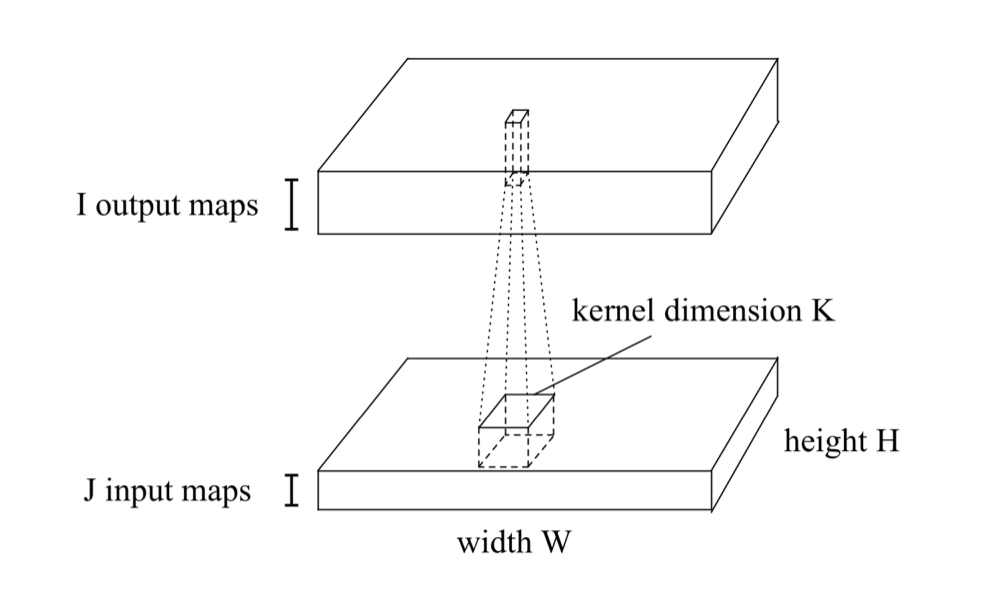
\includegraphics[width=0.75\textwidth]{img/size_conv_net}
\end{figure}
\begin{center}
    \begin{tabular}{c||c|c|}
        & fully connected layer & convolution layer \\
        \hline \hline
        \# output units & $WHI$ & $WHI$ \\
        \hline 
        \# weights & $W^2H^2IJ$ & $K^2IJ$ \\
        \hline
        \# connections & $W^2H^2IJ$ & $WHK^2IJ$ \\
        \hline
    \end{tabular}
\end{center}

\subsubsection{Rule of thumb on size}
\begin{itemize}
    \item Most of the units and connections are in the convolution layers, and
    \item Most of the weights are in the fully connected layers. 
\end{itemize}





















\newpage
\bibliographystyle{unsrt}
\bibliography{ref}
\end{document}
